\section{Experimentación Y Resultados}

\subsection{Casos de prueba}
   A continuación se listarán los casos utilizados y después se compararán los resultados.

	\begin{itemize}
		\item MOVIES: Este caso incluye 5797 páginas
		\item ABORTION: Este caso incluye 2293 páginas
		\item GENETIC: Este caso incluye 3468 páginas
		\item STANFORD: Este caso incluye 281903 páginas
		\item GOOGLE: Este caso incluye 916428 páginas
	\end{itemize}   

\subsection{Comparación de Normas}

En esta sección vamos a mostrar como evoluciona la norma Manhattan (también conocida como distancia L1) entre dos vectores a medida que se suceden las iteraciones.
La norma Manhattan es la distancia entre dos vectores, o en otras palabras, la suma de la diferencia coordenada a coordenada en modulo:

\begin{figure}[h!]
   \centering
    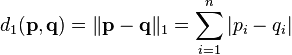
\includegraphics[width=0.5\textwidth]{imagenes/norma_manhattan.png}
\end{figure}


\subsubsection {PageRank}

Para evaluar el comportamiento de la norma manhattan variando la probabilidad del navegante aleatorio, el cual de ahora en más lo denotaremos como el parámetro \textbf{c}

Los casos de prueba se corrieron sin un limite entre normas pero si con un limite de 1000 iteraciones, ya que, según lo que investigamos, con un c 	$\approx$ 0.15 la matriz suele converger en un máximo de 50 iteraciones, que por lo que se puede observar suele ser proporcional esta relación a medida que aumenta el c.

A continuación se muestran los resultados para cuatro tests de como evoluciona la norma a lo largo de las iteraciones y como varía la misma con distintos c, y que luego discutiremos más adelante.
Cabe aclarar que expresamos los valores de la norma en escala logarítmica para una mejor visualización y para que se obtenga un mejor entendimiento de como disminuye de a varias magnitudes en cada iteración.


\begin{figure}
\begin{center}
       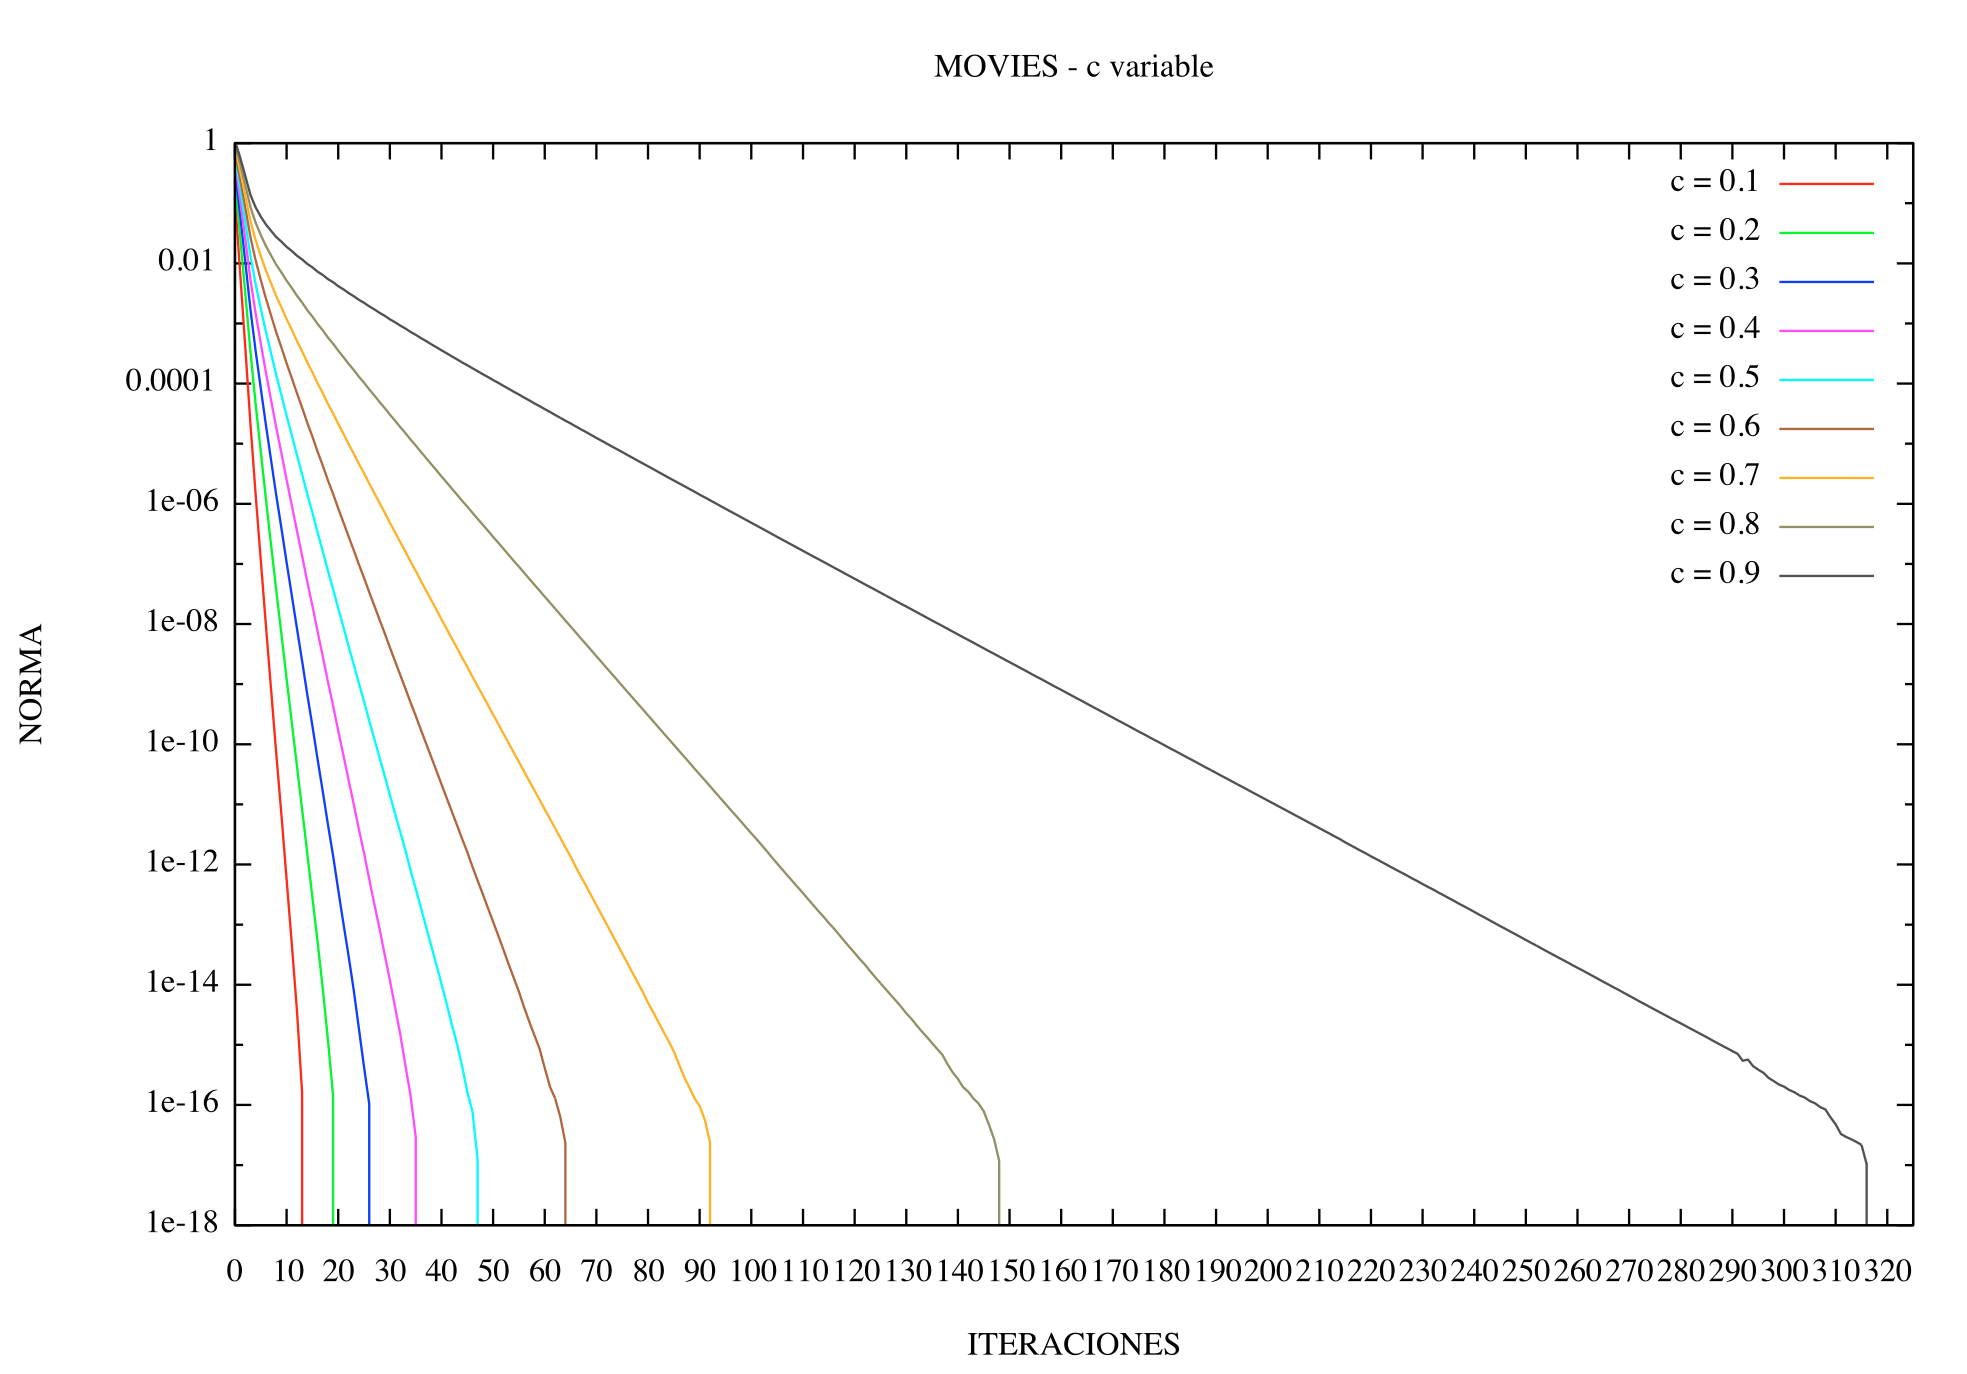
\includegraphics[scale=0.5]{imagenes/pagerank_movies_norma.png}
        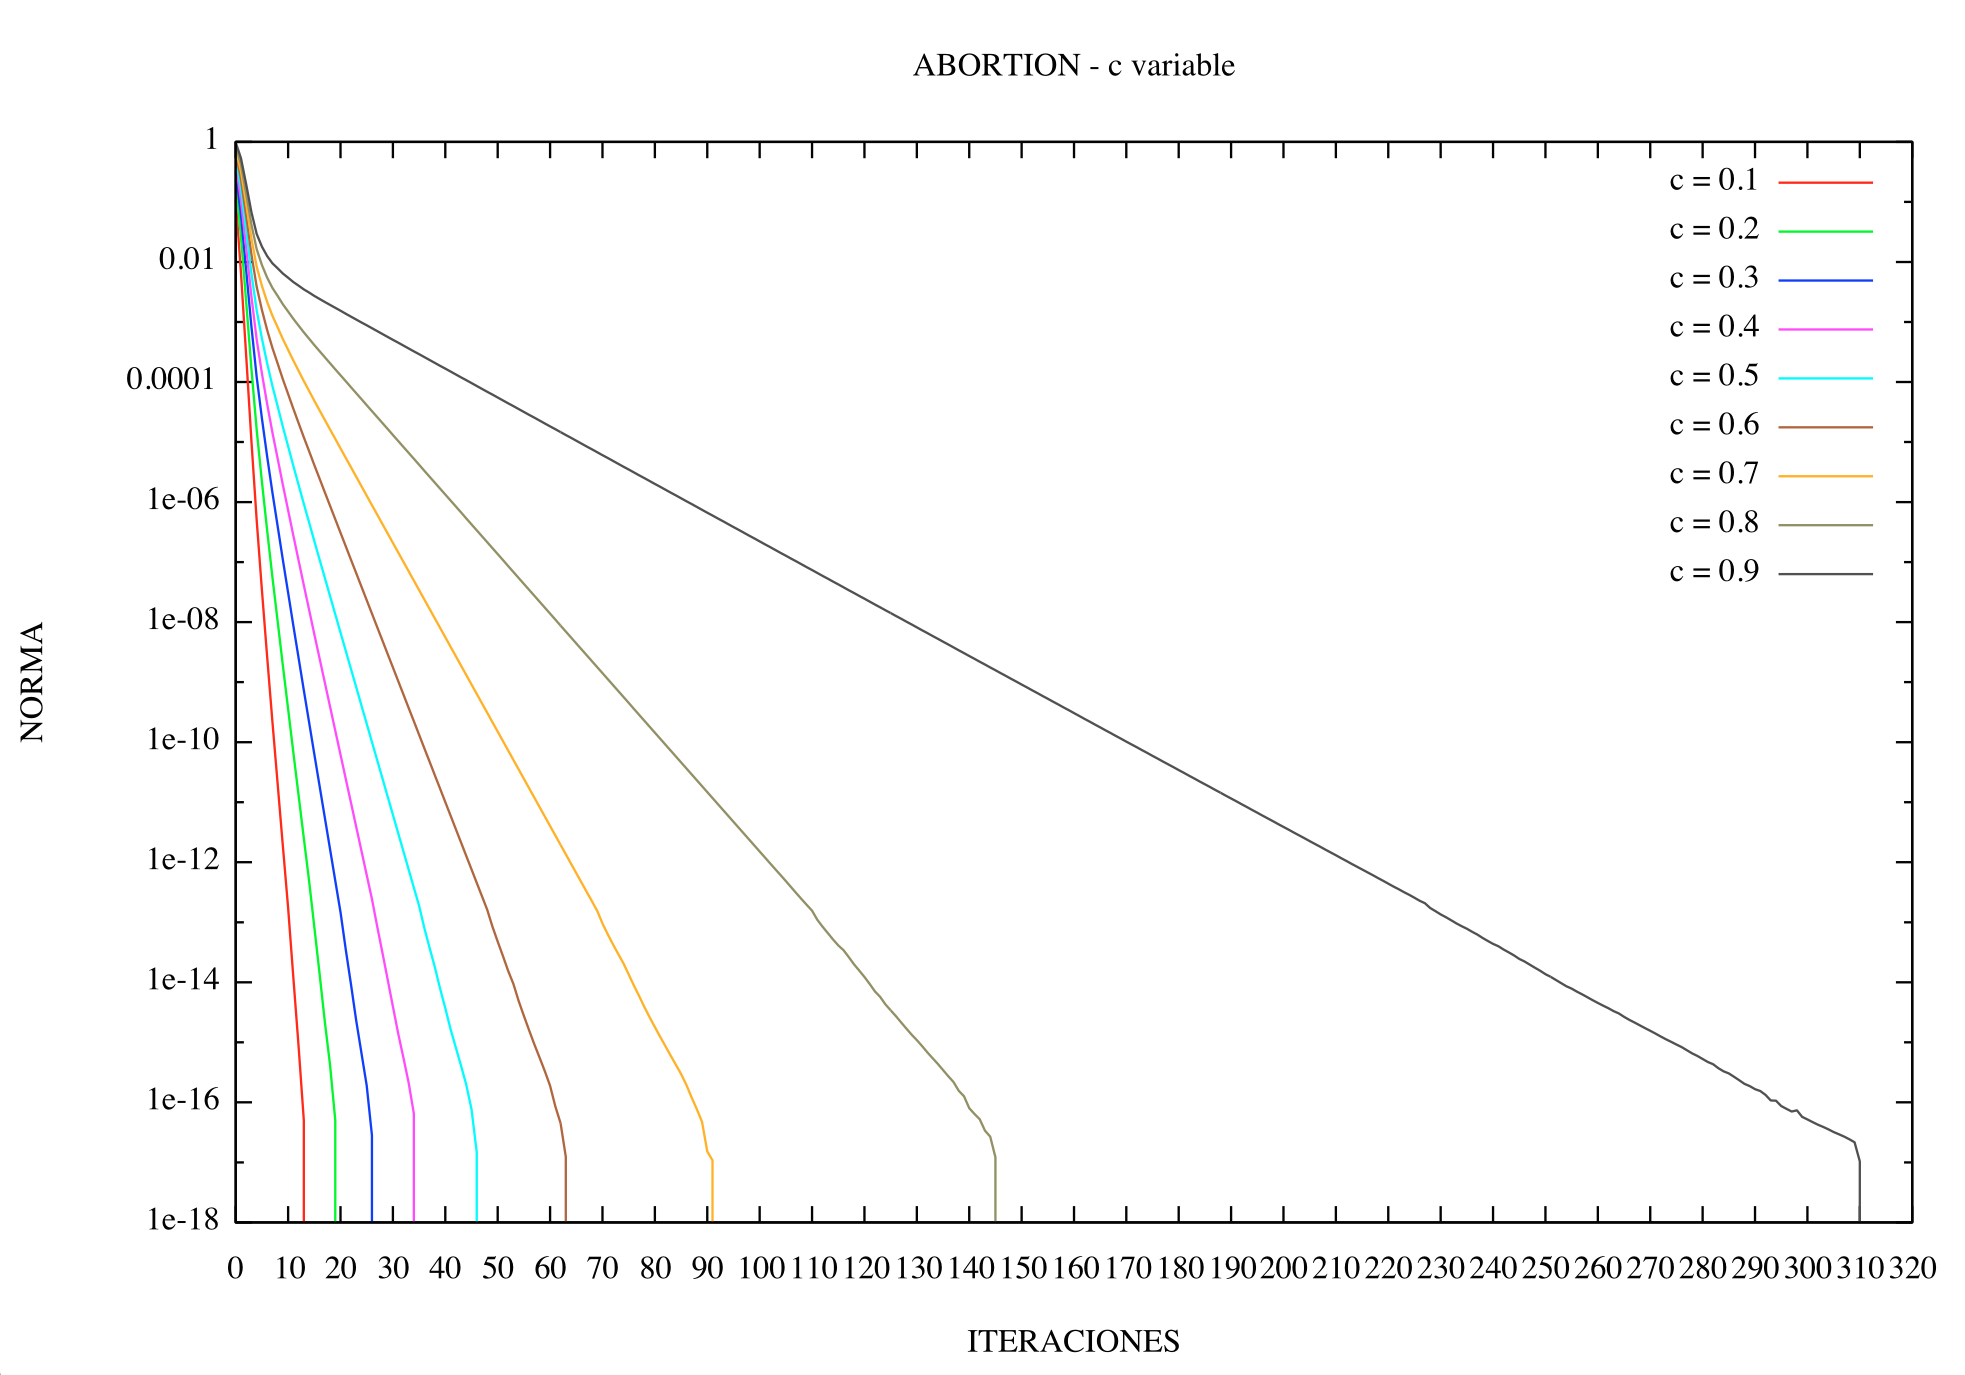
\includegraphics[scale=0.5]{imagenes/pagerank_abortion_norma.png}
       \end{center}
\end{figure}

\begin{figure}
\begin{center}
    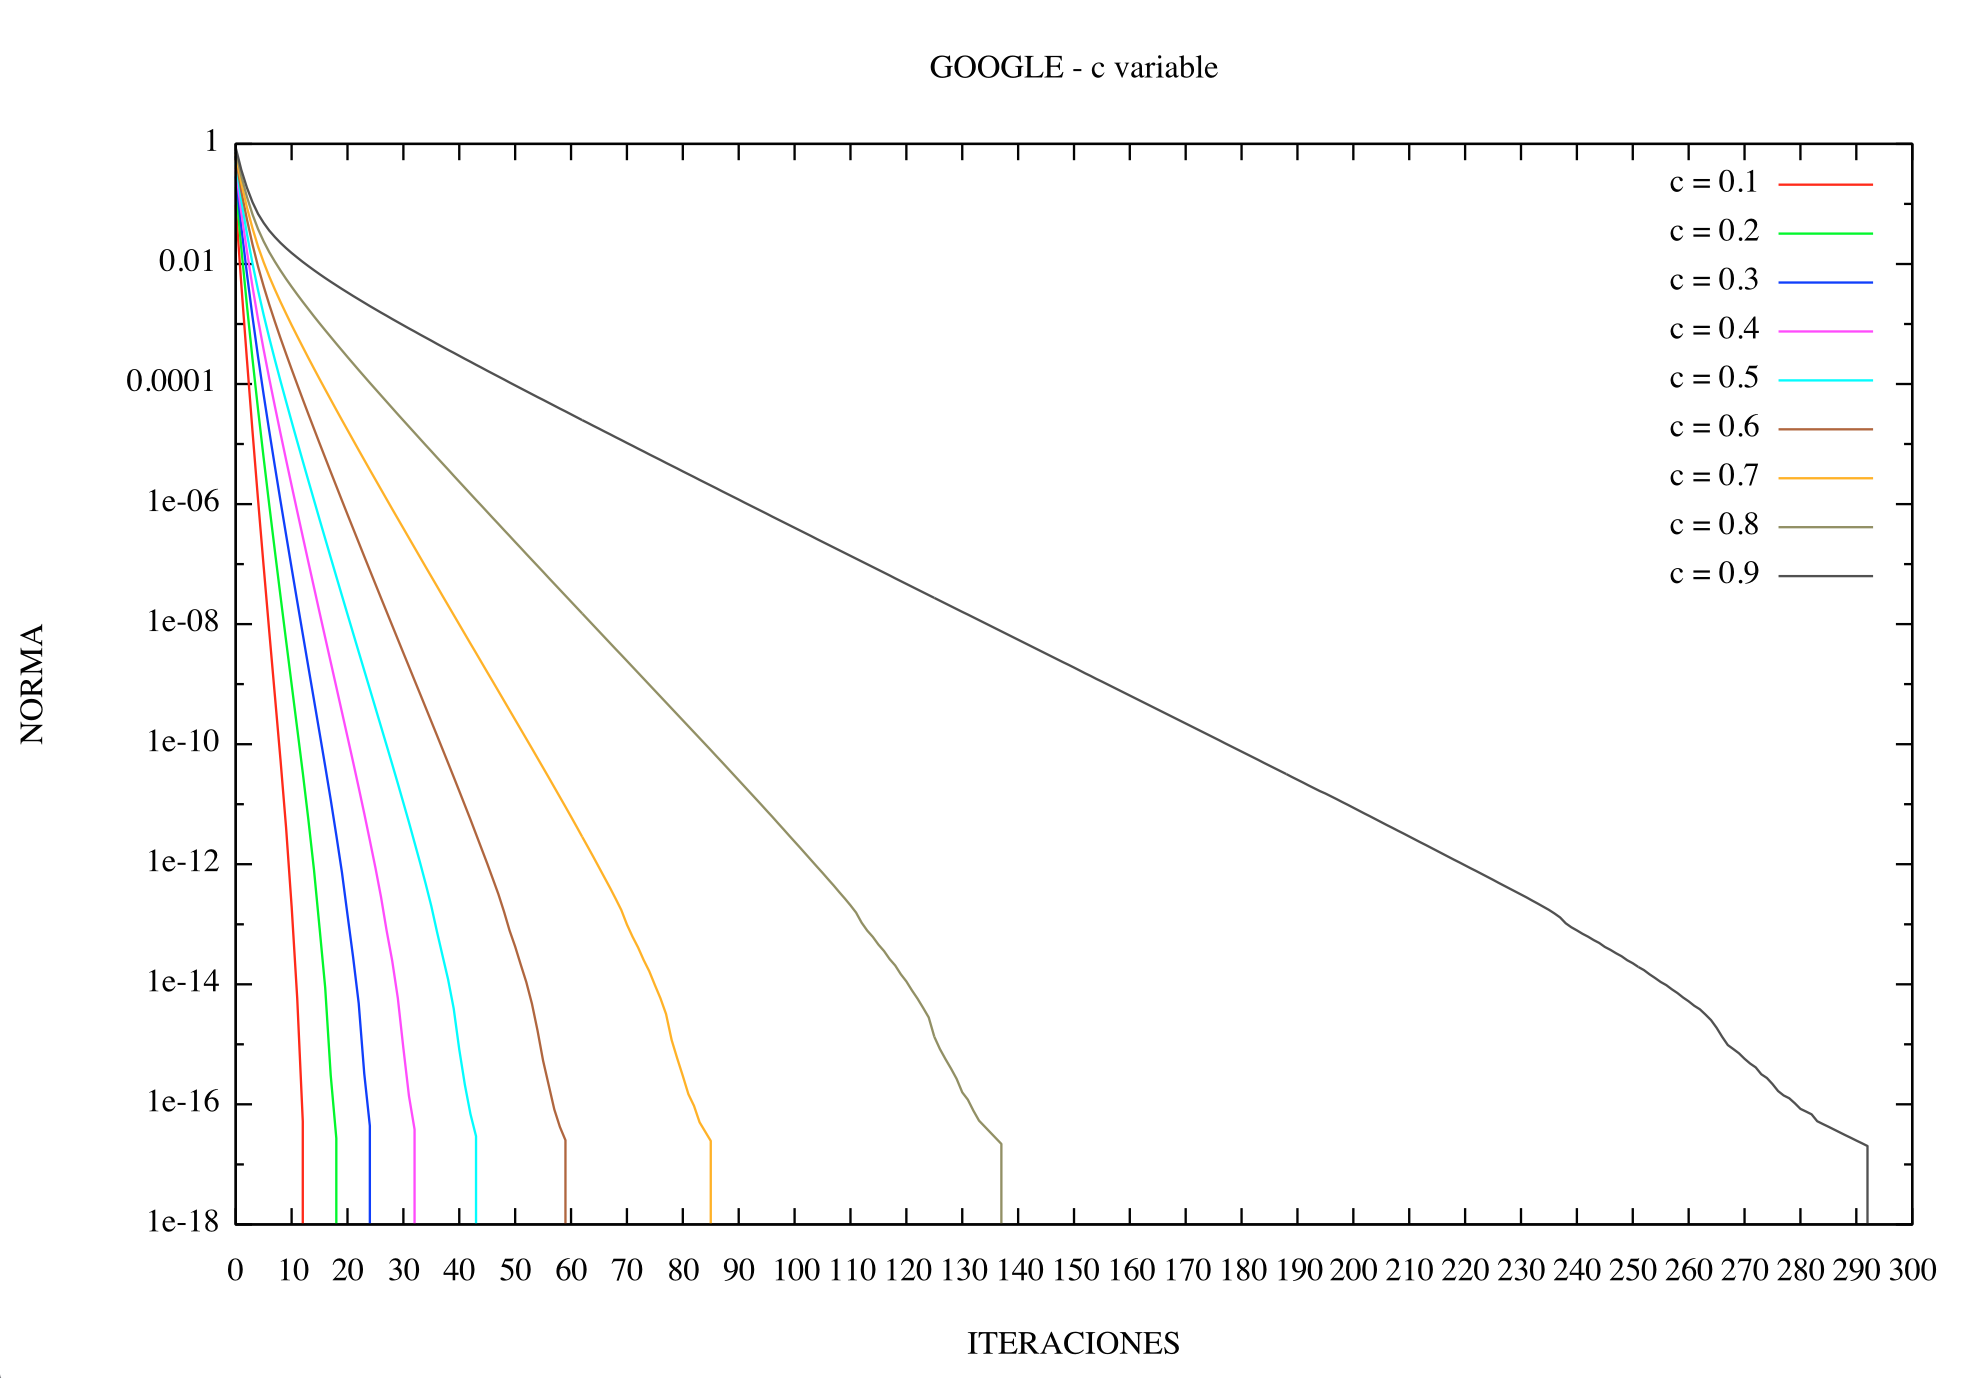
\includegraphics[scale=0.5]{imagenes/pagerank_google_norma.png}
  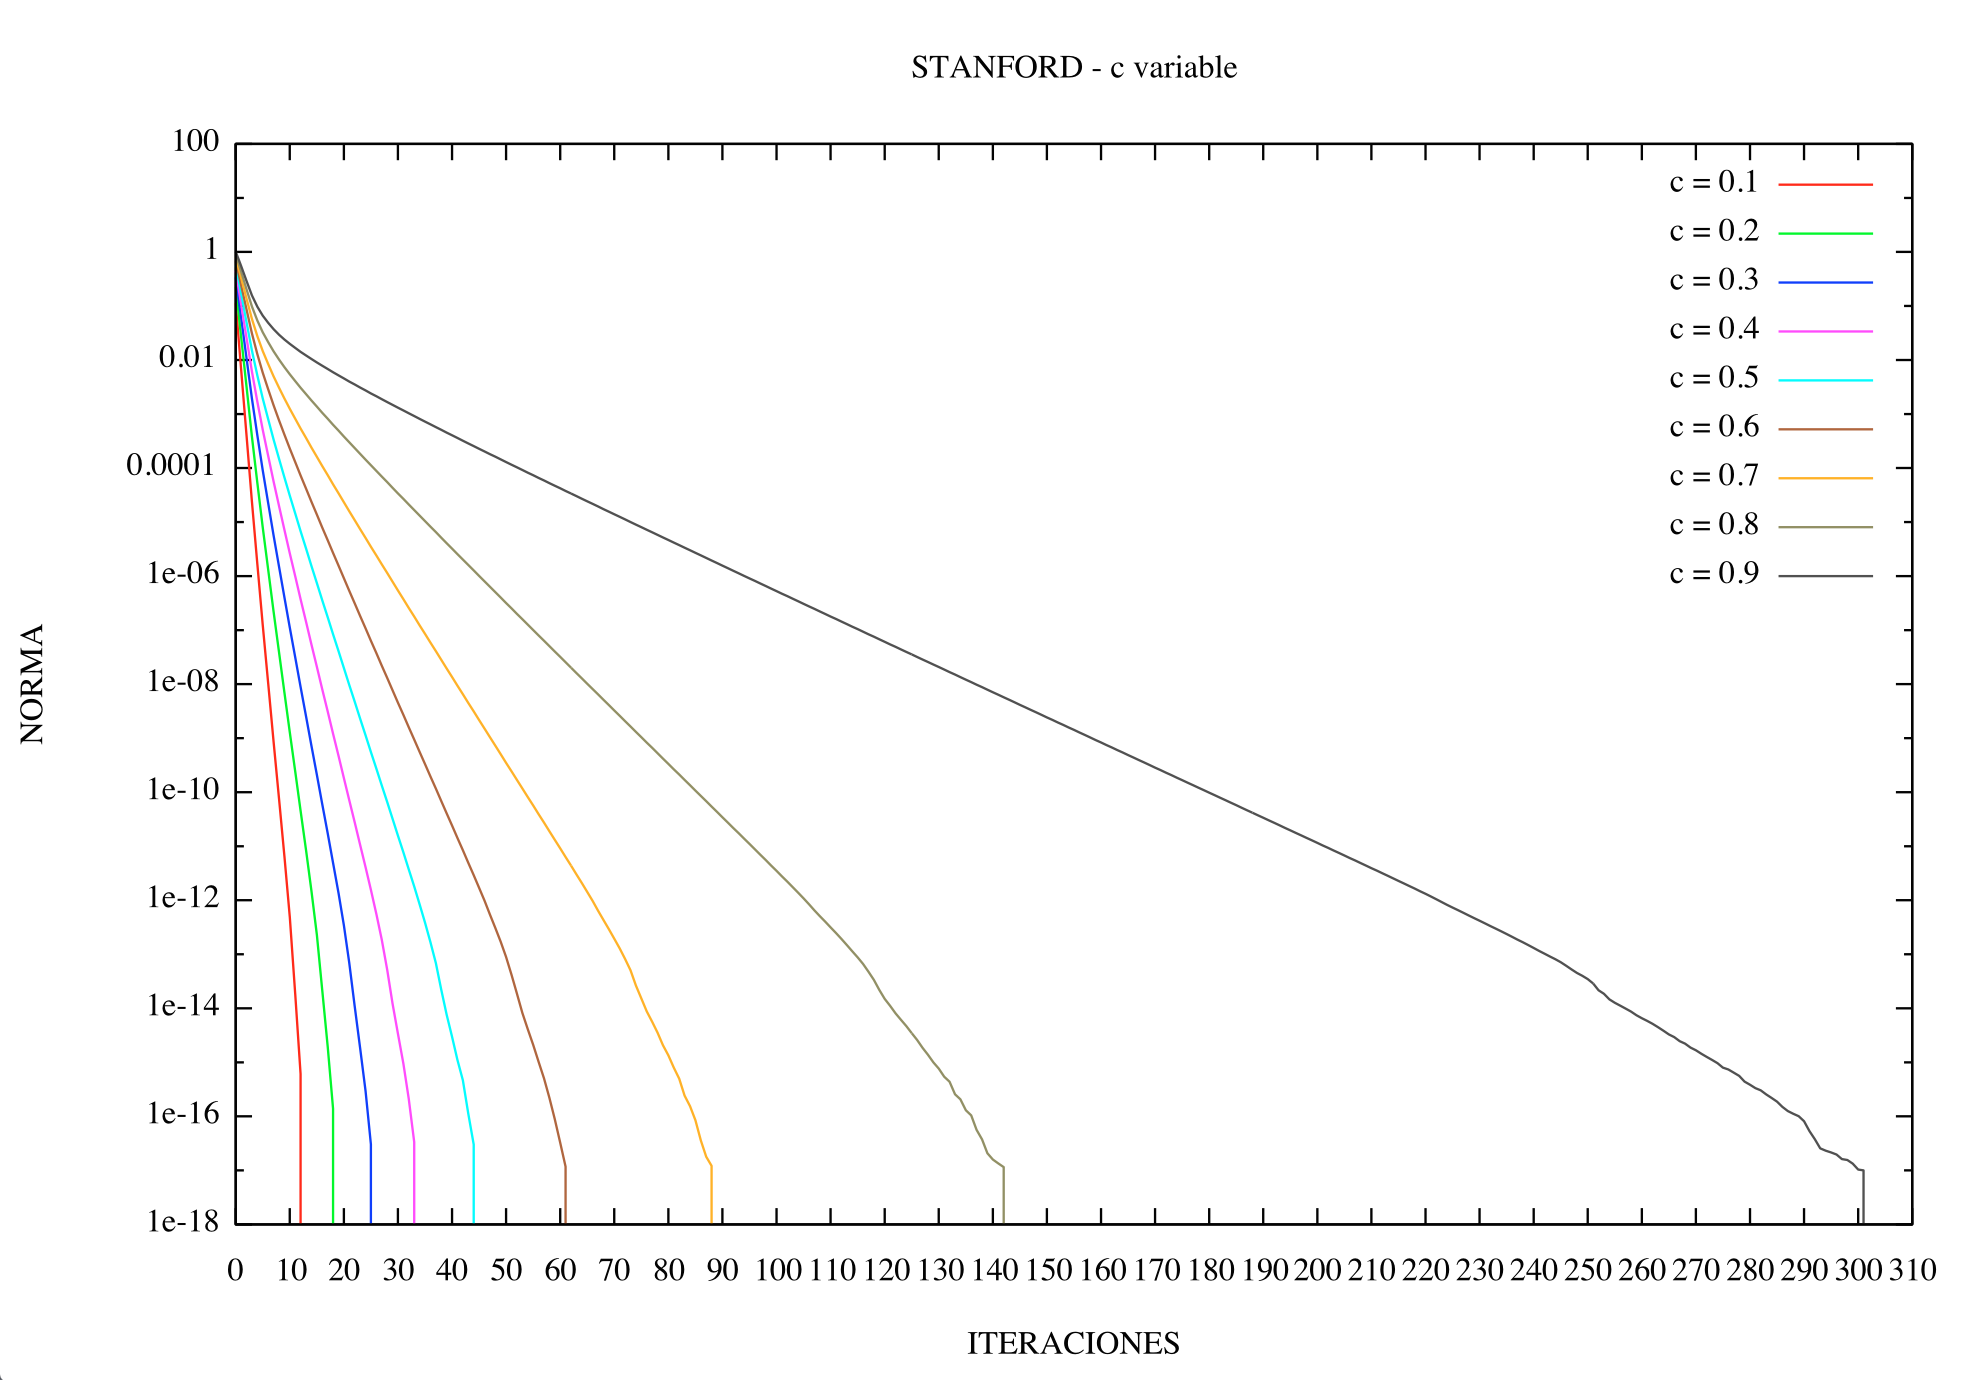
\includegraphics[scale=0.5]{imagenes/pagerank_stanford_norma.png}
    \end{center}
\end{figure}

\FloatBarrier




\subsubsection {HITS}


Estas corridas se hicieron para k= 100 ya que con esto alcanzaba para analizar los compartamientos deseados. La tolerancia en todos los casos fue de 0 ya que nos pareció mas interesante ver que tanto converge mas allá de que para nosotros una divergencia de 0.00001 ya es despreciable.

A continuación se muestran los resultados para cuatro instancias distintas, 3 medianas y una grande, de como evoluciona la norma a lo largo de las iteraciones en ambos vectores :
\begin{figure}[!htb]
\begin{center}
       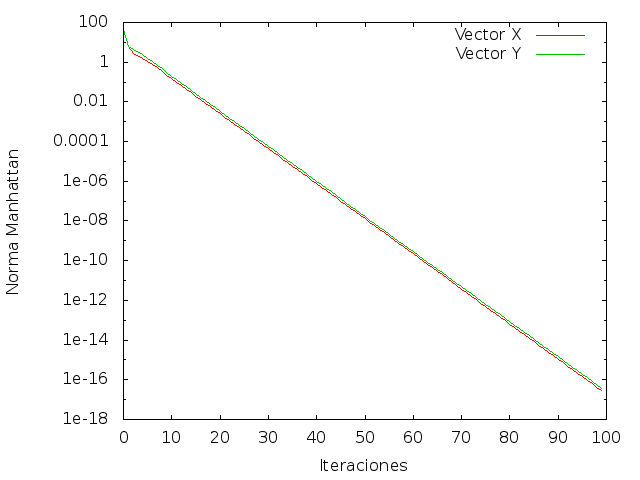
\includegraphics[scale=0.5]{imagenes/hits-abortion-expanded.png}
       \caption{Abortion expanded }
  \end{center}
\end{figure}
\begin{figure}[!htb]
\begin{center}
        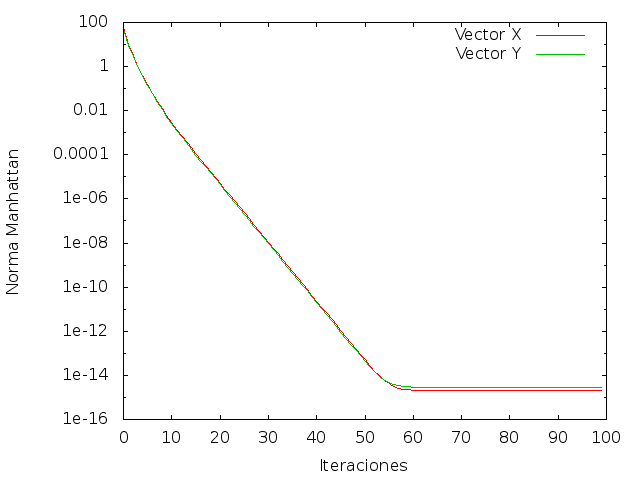
\includegraphics[scale=0.5]{imagenes/hits-genetic-expanded.png}
       \caption{Genetic expanded }
       \end{center}
\end{figure}

\begin{figure}[!htb]
\begin{center}
    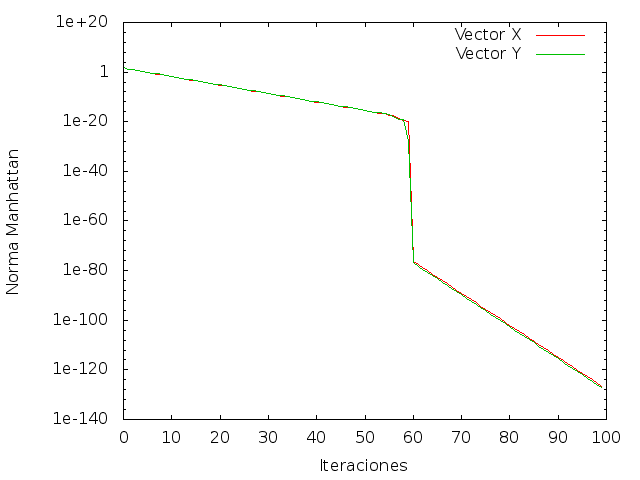
\includegraphics[scale=0.5]{imagenes/hits-movie.png}
    \caption{Movies expanded }
  \end{center}
\end{figure}
\begin{figure}[!htb]
\begin{center}
    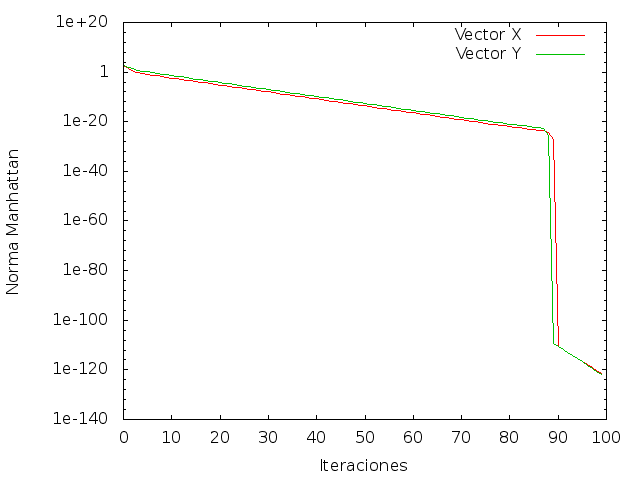
\includegraphics[scale=0.5]{imagenes/hits-stadfor.png}
    \caption{Standford}
    \end{center}
\end{figure}

\subsection{Comparación de Tiempos}

El siguiente gráfico muestra la evolución del tiempo de computo en función del tamaño de la red para cada algoritmo. La red utilizada en todos los casos es una red estrella en la que todos los nodos (o sitios) apuntan al primero de ellos. Utilizamos este tipo de grafo ya que en c++ es el más rápido y simple de crear teniendo en cuenta además que la forma del grafo no tiene un impacto de eficiencia en los algoritmos sino su tamaño en nodos y aristas es el que cambia el tiempo de ejecución. Por esto no nos pareció pertinente probar distintos tipos de grafos (arboles, completos, bipartito, etc) sin más bien el tamaño de los mismos.

 \begin{figure}[!htb]
\begin{center}
    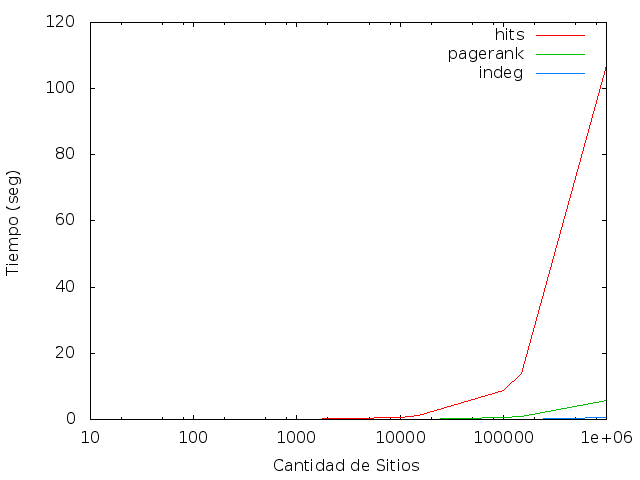
\includegraphics[scale=0.5]{imagenes/Tiempos.png}
    \caption{Tiempo de ejecución en función del tamaño de la red}
    \end{center}
\end{figure}



